\section{Literature Review}
\label{litreview}

\subsection{Inspiration from Human Learning}
\label{human}

Our brains process information through neurons, which combine many electrical inputs, called dendrites, into one output, the axon. These neurons are connected via synapses, which chemically transmit information via neurotransmitters. We learn by changing the amount of neurotransmitter released.

By connecting multiple neurons together, we allow for more complex outputs. Our cerebellum - the part of the brain that controls language, motor function, and cognitive learning - consists of roughly $10^{10}$ neurons, each connected to approximately $10000$ other neurons.

\subsection{Hebbian Theory}
\label{hebb}

To digitalise this biological structure of the brain, we need a mathematical model. The Hebbian Theory attempts to model this behaviour.

The Hebbian Theory suggests that if two neurons in space activate in phase - at the same time - the connection should strengthen between them. If in opposite phase, the connection should become weaker. No correlation between the activations should not affect the connection.

Hebbian learning tries to replicate learning in animals such that 
\begin{equation}
w_{ij}=x_ix_j 
\label{eq:hebb}
\end{equation}
where $w_{ij}$ is the weighted synapse between neuron $i$ and neuron $j$, and $x_i$ is the value at neuron $i$, at a given time in space. Linking this with the biological neuron, $x_i$ is the axon of $i$ - as with $j$ - and $w_{ij}$ is the strength of the synapse connecting the axon of $i$ to the dendrite of $j$.\\
We can rectify \eq{eq:hebb} to 
\begin{equation} 
\Delta w_{ij}=x_ix_j
\label{eq:dhebb}
\end{equation}
such that $w_{ij}$ changes based on its current state.

\subsection{Artificial Neural Networks}
\label{ann}

Unfortunately, we cannot directly use the Hebbian Theory for machine learning where we want the machine to learn a desired output for a specified input. This is because it doesn't know what the output is supposed to give, but rather how the input data is related - this type of learning is called unsupervised learning, which we will cover in Types of Learning.

\subsubsection{Neuron Model}
\label{model}

Consider a neuron $y$. There are many neurons connected to $y$, $x_1, x_2, \cdots, x_I$. The axon from $x_i$, $\text{A}(x_i)$, is connected to the $i^\text{th}$ dendrite of $y$, $\text{D}_i(y)$, via a weighted synapse $w_{i}$. Therefore $\text{D}_i(y)=w_i\text{A}(x_i)$. The dendrites of $y$ are combined to give the axon of $y$, $\text{A}(y)$.

The axon of $y$ can be simply modelled as 
\begin{equation}
\text{A}(y)=\sum^I_{i=1}\text{D}_i(y)
\end{equation}
or simply
\begin{equation} 
\text{A}(y)=\sum^I_{i=1}w_i\text{A}(x_i)
\label{eq:nmaxon}
\end{equation} 
Since we are dealing with just the axons of $x_i$ and $y$, we can simplify \eq{eq:nmaxon} as 
\begin{equation}
y=\sum^I_{i=1}w_ix_i
\label{eq:nmsimple}
\end{equation}

\subsubsection{Network Architecture}
\label{net}

$x_i$ and $y$ are neurons, which can be modeled as nodes

\begin{figure}[h]
\setlength{\unitlength}{0.14in} % selecting unit length
\centering % used for centering Figure
\begin{picture}(10,5) % picture environment with the size (dimensions)
 % 32 length units wide, and 15 units high.
\put(0.8, 0){$\vdots$}
\put(-0.1, 1.6){\framebox(2.2, 2.2){$x_i$}}
\put(0.8, 4.4){$\vdots$}

\put(7.9, 1.6){\framebox(2.2, 2.2){$y$}}

\end{picture}
\caption{Model of $x$ neurons and $y$ neuron}
\label{fig:xiy} 
\end{figure}

These neurons are connected via synapses, which can be modeled as a line connecting the neurons.

\begin{figure}[h]
\setlength{\unitlength}{0.14in}
\centering
\begin{picture}(10,5)


\put(0.8, 0){$\vdots$}
\put(-0.1, 1.6){\framebox(2.2, 2.2){$x_i$}}
\put(0.8, 4.4){$\vdots$}

\put(7.9, 1.6){\framebox(2.2, 2.2){$y$}}

\mline{1.5}{0.5}{6.0}{2.15}\mline{2.5}{2.65}{5.0}{0.0}\mline{1.5}{4.8}{6.0}{-2.15}

\end{picture}
\caption{Model of $x$ neurons connected to $y$ neuron with synapses}
\label{fig:xiys}
\end{figure}

We can add more neurons, $y_j$, from the same input neurons, $x_i$, using different synapses. This will increase the complexity of the neural network, allowing for more flexibility.

\begin{figure}[h]
\setlength{\unitlength}{0.14in}
\centering
\begin{picture}(10,5) 
\put(0.8, 0){$\vdots$}
\put(-0.1, 1.6){\framebox(2.2, 2.2){$x_i$}}
\put(0.8, 4.4){$\vdots$}

\put(8.8, 0){$\vdots$}
\put(7.9, 1.6){\framebox(2.2, 2.2){$y_j$}}
\put(8.8, 4.4){$\vdots$}

\mline{1.5}{0.5}{7.0}{0.0}
\mline{1.5}{0.5}{6.0}{2.15}
\mline{1.5}{0.5}{7.0}{4.3}

\mline{2.5}{2.65}{6.0}{2.15}
\mline{2.5}{2.65}{5.0}{0.0}
\mline{2.5}{2.65}{6.0}{-2.15}

\mline{1.5}{4.8}{7.0}{-4.3}
\mline{1.5}{4.8}{6.0}{-2.15}
\mline{1.5}{4.8}{7.0}{0.0}

\end{picture}
\caption{Model of $x$ neurons to $y$ neurons with synapses}
\label{fig:xiyjs}
\end{figure}

In a neural network, there are input, hidden, and output layers, where a layer contains neurons that activate at the same time at a specific depth within the network.

\begin{figure}[H]
\setlength{\unitlength}{0.14in}
\centering
\begin{picture}(34,5) 

\put(0.8, 0){$\vdots$}
\put(-0.1, 1.6){\framebox(2.2, 2.2){$x_i$}}
\put(0.8, 4.4){$\vdots$}

\put(8.4, 0){\reflectbox{$\ddots$}}
\put(8.4, 2.4){$\cdots$}
\put(8.4, 4.4){$\ddots$}

\put(16.8, 0){$\vdots$}
\put(15.9, 1.6){\framebox(2.2, 2.2){$h^L_n$}}
\put(16.8, 4.4){$\vdots$}

\put(24.4, 0){$\ddots$}
\put(24.4, 2.4){$\cdots$}
\put(24.4, 4.4){\reflectbox{$\ddots$}}

\put(32.8, 0){$\vdots$}
\put(31.9, 1.6){\framebox(2.2, 2.2){$y_j$}}
\put(32.8, 4.4){$\vdots$}

\mline{1.5}{0.5}{6.4}{0.0}
\mline{1.5}{0.5}{6.4}{2.15}
\mline{1.5}{0.5}{6.4}{4.3}

\mline{2.5}{2.65}{5.4}{2.15}
\mline{2.5}{2.65}{5.4}{0.0}
\mline{2.5}{2.65}{5.4}{-2.15}

\mline{1.5}{4.8}{6.4}{-4.3}
\mline{1.5}{4.8}{6.4}{-2.15}
\mline{1.5}{4.8}{6.4}{0.0}


\mline{10.1}{0.5}{6.4}{0.0}
\mline{10.1}{0.5}{5.4}{2.15}
\mline{10.1}{0.5}{6.4}{4.3}

\mline{10.1}{2.65}{6.4}{2.15}
\mline{10.1}{2.65}{5.4}{0.0}
\mline{10.1}{2.65}{6.4}{-2.15}

\mline{10.1}{4.8}{6.4}{-4.3}
\mline{10.1}{4.8}{5.4}{-2.15}
\mline{10.1}{4.8}{6.4}{0.0}


\mline{17.5}{0.5}{6.4}{0.0}
\mline{17.5}{0.5}{6.4}{2.15}
\mline{17.5}{0.5}{6.4}{4.3}

\mline{18.5}{2.65}{5.4}{2.15}
\mline{18.5}{2.65}{5.4}{0.0}
\mline{18.5}{2.65}{5.4}{-2.15}

\mline{17.5}{4.8}{6.4}{-4.3}
\mline{17.5}{4.8}{6.4}{-2.15}
\mline{17.5}{4.8}{6.4}{0.0}


\mline{26.1}{0.5}{6.4}{0.0}
\mline{26.1}{0.5}{5.4}{2.15}
\mline{26.1}{0.5}{6.4}{4.3}

\mline{26.1}{2.65}{6.4}{2.15}
\mline{26.1}{2.65}{5.4}{0.0}
\mline{26.1}{2.65}{6.4}{-2.15}

\mline{26.1}{4.8}{6.4}{-4.3}
\mline{26.1}{4.8}{5.4}{-2.15}
\mline{26.1}{4.8}{6.4}{0.0}


\end{picture}
\caption{Model of $x$ input neurons connected to $h^L$ neurons connected to $y$ output neurons}
\label{fig:xihLnyj}
\end{figure}

More layers allow for more complex functions, but if there are too many neurons, the neural network will overfit to the data, which essentially means it is memorising instead of learning. When it overfits to data, it is unlikely to produce similar results to input data that is slightly different. This is because when a neural network learns, it finds patterns in the data it is given, allowing it to be more flexible an give the correct output for a new given input.

\subsection{Gradient Descent}
\label{gd}

So far we have discussed how information is propagated forward through the network to produce an output, however there is no way we can change the weights of each synapse to achieve a different output, and thus learn.

Gradient Descent attempts to minimise the cost, $\nabla C$, of a neural network, which is a measure of how well it maps the target data. There are many ways of doing this, but for our simple feedforward architecture, the most common method is backpropagation.

\subsubsection{Backpropagation}
\label{backprop}

Backpropagation aims to change the weights of a neural network in the most efficient way such that the output of the neural network fits closer to the desired output, given a specified input. 

Consider the following neural network.

\begin{figure}[h]
\setlength{\unitlength}{0.14in}
\centering
\begin{picture}(10,5) 

\put(-0.1, 1.6){\framebox(2.2, 2.2){$X$}}
\put(4.6, 3){$w$}
\put(7.9, 1.6){\framebox(2.2, 2.2){$O$}}

\mline{2.5}{2.65}{5.0}{0.0}

\end{picture}
\caption{Model of neuron $X$ connected to neuron $O$ with a weighted synapse $w$}
\label{fig:XwO}
\end{figure}

We can describe the how close the output, $O$, is to the target, $Y$, with the cost, $C$, which is equal to the square of the difference of $O$ and $Y$. We square this value so that the cost is positive, and it is continuously differentiable, which will prove very useful later on. $$C=(O-Y)^2$$

We can make a graph of how $w$ effects $C$, so we can find what weight gives the minimum cost, and therefore the closest output to our target. 

\begin{figure}[h]
\setlength{\unitlength}{0.14in}
\centering
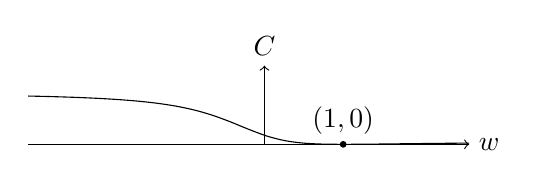
\begin{tikzpicture}
\draw[->] (-3,0) -- (2.6,0) node[right] {$w$};
\draw[->] (0,0) -- (0,1) node[above] {$C$};
\draw[scale=1.0,domain=-3:2.6,smooth,variable=\x,black] plot ({\x},{(((1/(1+e^(-(\x*-3))))-(1/(1+e^(-(-3)))))^2+((1/(1+e^(-(\x*-2))))-(1/(1+e^(-(-2)))))^2+((1/(1+e^(-(\x*-1))))-(1/(1+e^(-(-1)))))^2+((1/(1+e^(-(\x*0))))-(1/(1+e^(-(0)))))^2+((1/(1+e^(-(\x*1))))-(1/(1+e^(-(1)))))^2+((1/(1+e^(-(\x*2))))-(1/(1+e^(-(2)))))^2+((1/(1+e^(-(\x*3))))-(1/(1+e^(-(3)))))^2)/7});
\filldraw[black] (1,0) circle (1pt) node[anchor=south] {$(1,0)$};
\end{tikzpicture}
\caption{A graph of $C$ against $w$}
\label{fig:Cw}
\end{figure}

We know that where $w=1$, we achieve a cost of $0$, so the output is equal to the input. However, we do not want to iterate through all possible weights in a neural network to find the minimum cost, as that is very computationally expensive. Instead, we should start at a random $w$, say $-1$, and take small steps downhill, hence gradient descent. 

\begin{figure}[h]
\setlength{\unitlength}{0.14in}
\centering
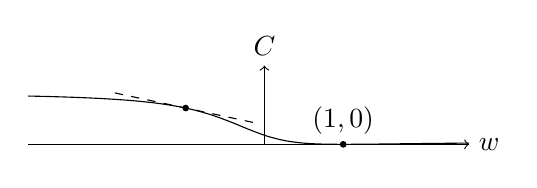
\begin{tikzpicture}
\draw[->] (-3,0) -- (2.6,0) node[right] {$w$};
\draw[->] (0,0) -- (0,1) node[above] {$C$};
\draw[scale=1.0,domain=-3:2.6,smooth,variable=\x,black] plot({\x},{(((1/(1+e^(-(\x*-3))))-(1/(1+e^(-(-3)))))^2+((1/(1+e^(-(\x*-2))))-(1/(1+e^(-(-2)))))^2+((1/(1+e^(-(\x*-1))))-(1/(1+e^(-(-1)))))^2+((1/(1+e^(-(\x*0))))-(1/(1+e^(-(0)))))^2+((1/(1+e^(-(\x*1))))-(1/(1+e^(-(1)))))^2+((1/(1+e^(-(\x*2))))-(1/(1+e^(-(2)))))^2+((1/(1+e^(-(\x*3))))-(1/(1+e^(-(3)))))^2)/7});
\draw[scale=1.0,domain=-1.9:-0.1,dashed,variable=\x,black] plot({\x},{-0.21340427*\x+0.46082-0.21340427});
\filldraw[black] (1,0) circle (1pt) node[anchor=south] {$(1,0)$};
\filldraw[black] (-1,0.46082) circle (1pt);
\end{tikzpicture}
\caption{A graph of $C$ against $w$ showing the gradient at $w=-1$}
\label{fig:Cwm}
\end{figure}
We can decrease the cost, $C$, by repeatedly changing $w$ proportionally to the negative gradient at $w$, or 
\begin{equation}
\Delta w=-\alpha\frac{\partial C}{\partial w}
\end{equation}
where $\alpha$ is the learning rate, which is essentially how big of a step in the given direction you take - too small, and it will take too long finding the minima - too large, and you will overshoot the minima, almost rocking back and forth.

Now, all we need to do is find the gradient.

\subsubsection{Using the Chain Rule}
\label{chain}

Using \fig{fig:XwO}, we can express $C$ as a series of functions 

$$C=(O-Y)^2$$
$$O=\sigma(z)$$
$$z=wX$$

Using the chain rule, we can equate
\begin{equation}
\frac{\partial C}{\partial w}=\frac{\partial C}{\partial O}\frac{\partial O}{\partial z}\frac{\partial z}{\partial w}=2(O-Y)\sigma'(z)X
\label{eq:crw}
\end{equation}
\eq{eq:crw} only works for \fig{fig:XwO}, so we need a more general model. 

Since we are dealing with multiple neurons, weights, and layers, we need a syntax to index these:

$x^L_i$ represents the $i^\text{th}$ neuron in layer $L$;
$Y^L_i$ represents the target for $x^L_i$;
$n_L$ represents the number of neurons in layer $L$;
$w^L_{ij}$ represents the weight of the synapse connected to the $i^\text{th}$ neuron in layer $L$, from the $j^\text{th}$ neuron in layer $L-1$

Consider the following

\begin{figure}[h]
\setlength{\unitlength}{0.14in}
\centering
\begin{picture}(16,5) 

\put(0.8, 0){$\vdots$}
\put(-0.1, 1.6){\framebox(2.2, 2.2){$Y^{L-1}_k$}}
\put(0.8, 4.4){$\vdots$}

\put(3.8, 0){$\vdots$}
\put(2.9, 1.6){\framebox(2.2, 2.2){$x^{L-1}_k$}}
\put(3.8, 4.4){$\vdots$}

\put(11.8, 0){$\vdots$}
\put(10.9, 1.6){\framebox(2.2, 2.2){$x^{L}_j$}}
\put(11.8, 4.4){$\vdots$}

\put(14.8, 0){$\vdots$}
\put(13.9, 1.6){\framebox(2.2, 2.2){$Y^{L}_j$}}
\put(14.8, 4.4){$\vdots$}

\mline{4.5}{0.5}{7.0}{0.0}
\mline{4.5}{0.5}{6.0}{2.15}
\mline{4.5}{0.5}{7.0}{4.3}

\mline{5.5}{2.65}{6.0}{2.15}
\mline{5.5}{2.65}{5.0}{0.0}
\mline{5.5}{2.65}{6.0}{-2.15}

\mline{4.5}{4.8}{7.0}{-4.3}
\mline{4.5}{4.8}{6.0}{-2.15}
\mline{4.5}{4.8}{7.0}{0.0}

\end{picture}
\caption{}
\label{fig:}
\end{figure}
The cost from multiple outputs is the sum of each cost of the output to the corresponding output $$C=\sum_{j=0}^{n_L-1}{(x^L_j-Y_j)^2}$$ The output remains similar to before $$x^L_j=\sigma(z^L_j)$$ where $$z^L_j=\sum_{k=0}^{n_{L-1}-1}w_{jk}^Lx_{k}^{L-1}$$

We can reevaluate the gradient again using the chain rule 

\begin{equation}
\frac{\partial C}{\partial w_{jk}^L}=\frac{\partial C}{\partial x^L_j}\frac{\partial x^L_j}{\partial z^L_j}\frac{\partial z^L_j}{\partial w_{jk}^L}=2(x_{j}^{L}-Y^L_j)\sigma'(z^L_j)x^{L-1}_k
\label{eq:gcrw}
\end{equation}

To find out what $x^{L-1}_k$ should be, $Y^{L-1}_k$, we can use the chain rule against $x^{L-1}_k$ instead of $w_{jk}^L$

\begin{equation}
Y^{L-1}_k=\frac{\partial C}{\partial x^{L-1}_k}=\frac{\partial C}{\partial x^L_j}\frac{\partial x^L_j}{\partial z^L_j}\frac{\partial z^L_j}{\partial x^{L-1}_k}=2(x_{j}^{L}-Y^L_j)\sigma'(z^L_j)w_{jk}^L
\label{eq:gcrY}
\end{equation}

We can then repeat this for each layer going backwards, until all the weights have been rectified to decrease the cost in the most efficient way possible, $\nabla C$. If we repeat this process for each $\{X_i,Y_i\}$ in training set $T$, we would have trained a function to fit to $T$.